% Options for packages loaded elsewhere
\PassOptionsToPackage{unicode}{hyperref}
\PassOptionsToPackage{hyphens}{url}
\PassOptionsToPackage{dvipsnames,svgnames,x11names}{xcolor}
%
\documentclass[
  letterpaper,
  DIV=11,
  numbers=noendperiod]{scrartcl}

\usepackage{amsmath,amssymb}
\usepackage{lmodern}
\usepackage{iftex}
\ifPDFTeX
  \usepackage[T1]{fontenc}
  \usepackage[utf8]{inputenc}
  \usepackage{textcomp} % provide euro and other symbols
\else % if luatex or xetex
  \usepackage{unicode-math}
  \defaultfontfeatures{Scale=MatchLowercase}
  \defaultfontfeatures[\rmfamily]{Ligatures=TeX,Scale=1}
\fi
% Use upquote if available, for straight quotes in verbatim environments
\IfFileExists{upquote.sty}{\usepackage{upquote}}{}
\IfFileExists{microtype.sty}{% use microtype if available
  \usepackage[]{microtype}
  \UseMicrotypeSet[protrusion]{basicmath} % disable protrusion for tt fonts
}{}
\makeatletter
\@ifundefined{KOMAClassName}{% if non-KOMA class
  \IfFileExists{parskip.sty}{%
    \usepackage{parskip}
  }{% else
    \setlength{\parindent}{0pt}
    \setlength{\parskip}{6pt plus 2pt minus 1pt}}
}{% if KOMA class
  \KOMAoptions{parskip=half}}
\makeatother
\usepackage{xcolor}
\setlength{\emergencystretch}{3em} % prevent overfull lines
\setcounter{secnumdepth}{5}
% Make \paragraph and \subparagraph free-standing
\ifx\paragraph\undefined\else
  \let\oldparagraph\paragraph
  \renewcommand{\paragraph}[1]{\oldparagraph{#1}\mbox{}}
\fi
\ifx\subparagraph\undefined\else
  \let\oldsubparagraph\subparagraph
  \renewcommand{\subparagraph}[1]{\oldsubparagraph{#1}\mbox{}}
\fi

\usepackage{color}
\usepackage{fancyvrb}
\newcommand{\VerbBar}{|}
\newcommand{\VERB}{\Verb[commandchars=\\\{\}]}
\DefineVerbatimEnvironment{Highlighting}{Verbatim}{commandchars=\\\{\}}
% Add ',fontsize=\small' for more characters per line
\usepackage{framed}
\definecolor{shadecolor}{RGB}{241,243,245}
\newenvironment{Shaded}{\begin{snugshade}}{\end{snugshade}}
\newcommand{\AlertTok}[1]{\textcolor[rgb]{0.68,0.00,0.00}{#1}}
\newcommand{\AnnotationTok}[1]{\textcolor[rgb]{0.37,0.37,0.37}{#1}}
\newcommand{\AttributeTok}[1]{\textcolor[rgb]{0.40,0.45,0.13}{#1}}
\newcommand{\BaseNTok}[1]{\textcolor[rgb]{0.68,0.00,0.00}{#1}}
\newcommand{\BuiltInTok}[1]{\textcolor[rgb]{0.00,0.23,0.31}{#1}}
\newcommand{\CharTok}[1]{\textcolor[rgb]{0.13,0.47,0.30}{#1}}
\newcommand{\CommentTok}[1]{\textcolor[rgb]{0.37,0.37,0.37}{#1}}
\newcommand{\CommentVarTok}[1]{\textcolor[rgb]{0.37,0.37,0.37}{\textit{#1}}}
\newcommand{\ConstantTok}[1]{\textcolor[rgb]{0.56,0.35,0.01}{#1}}
\newcommand{\ControlFlowTok}[1]{\textcolor[rgb]{0.00,0.23,0.31}{#1}}
\newcommand{\DataTypeTok}[1]{\textcolor[rgb]{0.68,0.00,0.00}{#1}}
\newcommand{\DecValTok}[1]{\textcolor[rgb]{0.68,0.00,0.00}{#1}}
\newcommand{\DocumentationTok}[1]{\textcolor[rgb]{0.37,0.37,0.37}{\textit{#1}}}
\newcommand{\ErrorTok}[1]{\textcolor[rgb]{0.68,0.00,0.00}{#1}}
\newcommand{\ExtensionTok}[1]{\textcolor[rgb]{0.00,0.23,0.31}{#1}}
\newcommand{\FloatTok}[1]{\textcolor[rgb]{0.68,0.00,0.00}{#1}}
\newcommand{\FunctionTok}[1]{\textcolor[rgb]{0.28,0.35,0.67}{#1}}
\newcommand{\ImportTok}[1]{\textcolor[rgb]{0.00,0.46,0.62}{#1}}
\newcommand{\InformationTok}[1]{\textcolor[rgb]{0.37,0.37,0.37}{#1}}
\newcommand{\KeywordTok}[1]{\textcolor[rgb]{0.00,0.23,0.31}{#1}}
\newcommand{\NormalTok}[1]{\textcolor[rgb]{0.00,0.23,0.31}{#1}}
\newcommand{\OperatorTok}[1]{\textcolor[rgb]{0.37,0.37,0.37}{#1}}
\newcommand{\OtherTok}[1]{\textcolor[rgb]{0.00,0.23,0.31}{#1}}
\newcommand{\PreprocessorTok}[1]{\textcolor[rgb]{0.68,0.00,0.00}{#1}}
\newcommand{\RegionMarkerTok}[1]{\textcolor[rgb]{0.00,0.23,0.31}{#1}}
\newcommand{\SpecialCharTok}[1]{\textcolor[rgb]{0.37,0.37,0.37}{#1}}
\newcommand{\SpecialStringTok}[1]{\textcolor[rgb]{0.13,0.47,0.30}{#1}}
\newcommand{\StringTok}[1]{\textcolor[rgb]{0.13,0.47,0.30}{#1}}
\newcommand{\VariableTok}[1]{\textcolor[rgb]{0.07,0.07,0.07}{#1}}
\newcommand{\VerbatimStringTok}[1]{\textcolor[rgb]{0.13,0.47,0.30}{#1}}
\newcommand{\WarningTok}[1]{\textcolor[rgb]{0.37,0.37,0.37}{\textit{#1}}}

\providecommand{\tightlist}{%
  \setlength{\itemsep}{0pt}\setlength{\parskip}{0pt}}\usepackage{longtable,booktabs,array}
\usepackage{calc} % for calculating minipage widths
% Correct order of tables after \paragraph or \subparagraph
\usepackage{etoolbox}
\makeatletter
\patchcmd\longtable{\par}{\if@noskipsec\mbox{}\fi\par}{}{}
\makeatother
% Allow footnotes in longtable head/foot
\IfFileExists{footnotehyper.sty}{\usepackage{footnotehyper}}{\usepackage{footnote}}
\makesavenoteenv{longtable}
\usepackage{graphicx}
\makeatletter
\def\maxwidth{\ifdim\Gin@nat@width>\linewidth\linewidth\else\Gin@nat@width\fi}
\def\maxheight{\ifdim\Gin@nat@height>\textheight\textheight\else\Gin@nat@height\fi}
\makeatother
% Scale images if necessary, so that they will not overflow the page
% margins by default, and it is still possible to overwrite the defaults
% using explicit options in \includegraphics[width, height, ...]{}
\setkeys{Gin}{width=\maxwidth,height=\maxheight,keepaspectratio}
% Set default figure placement to htbp
\makeatletter
\def\fps@figure{htbp}
\makeatother
\newlength{\cslhangindent}
\setlength{\cslhangindent}{1.5em}
\newlength{\csllabelwidth}
\setlength{\csllabelwidth}{3em}
\newlength{\cslentryspacingunit} % times entry-spacing
\setlength{\cslentryspacingunit}{\parskip}
\newenvironment{CSLReferences}[2] % #1 hanging-ident, #2 entry spacing
 {% don't indent paragraphs
  \setlength{\parindent}{0pt}
  % turn on hanging indent if param 1 is 1
  \ifodd #1
  \let\oldpar\par
  \def\par{\hangindent=\cslhangindent\oldpar}
  \fi
  % set entry spacing
  \setlength{\parskip}{#2\cslentryspacingunit}
 }%
 {}
\usepackage{calc}
\newcommand{\CSLBlock}[1]{#1\hfill\break}
\newcommand{\CSLLeftMargin}[1]{\parbox[t]{\csllabelwidth}{#1}}
\newcommand{\CSLRightInline}[1]{\parbox[t]{\linewidth - \csllabelwidth}{#1}\break}
\newcommand{\CSLIndent}[1]{\hspace{\cslhangindent}#1}

\KOMAoption{captions}{tableheading}
\makeatletter
\makeatother
\makeatletter
\makeatother
\makeatletter
\@ifpackageloaded{caption}{}{\usepackage{caption}}
\AtBeginDocument{%
\ifdefined\contentsname
  \renewcommand*\contentsname{Table of contents}
\else
  \newcommand\contentsname{Table of contents}
\fi
\ifdefined\listfigurename
  \renewcommand*\listfigurename{List of Figures}
\else
  \newcommand\listfigurename{List of Figures}
\fi
\ifdefined\listtablename
  \renewcommand*\listtablename{List of Tables}
\else
  \newcommand\listtablename{List of Tables}
\fi
\ifdefined\figurename
  \renewcommand*\figurename{Figure}
\else
  \newcommand\figurename{Figure}
\fi
\ifdefined\tablename
  \renewcommand*\tablename{Table}
\else
  \newcommand\tablename{Table}
\fi
}
\@ifpackageloaded{float}{}{\usepackage{float}}
\floatstyle{ruled}
\@ifundefined{c@chapter}{\newfloat{codelisting}{h}{lop}}{\newfloat{codelisting}{h}{lop}[chapter]}
\floatname{codelisting}{Listing}
\newcommand*\listoflistings{\listof{codelisting}{List of Listings}}
\makeatother
\makeatletter
\@ifpackageloaded{caption}{}{\usepackage{caption}}
\@ifpackageloaded{subcaption}{}{\usepackage{subcaption}}
\makeatother
\makeatletter
\@ifpackageloaded{tcolorbox}{}{\usepackage[many]{tcolorbox}}
\makeatother
\makeatletter
\@ifundefined{shadecolor}{\definecolor{shadecolor}{rgb}{.97, .97, .97}}
\makeatother
\makeatletter
\makeatother
\ifLuaTeX
  \usepackage{selnolig}  % disable illegal ligatures
\fi
\IfFileExists{bookmark.sty}{\usepackage{bookmark}}{\usepackage{hyperref}}
\IfFileExists{xurl.sty}{\usepackage{xurl}}{} % add URL line breaks if available
\urlstyle{same} % disable monospaced font for URLs
\hypersetup{
  pdftitle={AI for Shrubland Identification and Mapping},
  pdfauthor={Michael J Mahoney1,; Lucas K Johnson1; Colin M Beier2},
  colorlinks=true,
  linkcolor={blue},
  filecolor={Maroon},
  citecolor={Blue},
  urlcolor={Blue},
  pdfcreator={LaTeX via pandoc}}

\title{AI for Shrubland Identification and Mapping}
\author{Michael J Mahoney\textsuperscript{1,*} \and Lucas K Johnson\textsuperscript{1} \and Colin M Beier\textsuperscript{2}}
\date{}

\begin{document}
\maketitle
\ifdefined\Shaded\renewenvironment{Shaded}{\begin{tcolorbox}[frame hidden, interior hidden, borderline west={3pt}{0pt}{shadecolor}, boxrule=0pt, enhanced, breakable, sharp corners]}{\end{tcolorbox}}\fi

\textsuperscript{1} Graduate Program in Environmental Science, State
University of New York College of Environmental Science and Forestry, 1
Forestry Drive, Syracuse, NY, 13210\\
\textsuperscript{2} Department of Sustainable Resources Management,
State University of New York College of Environmental Science and
Forestry, 1 Forestry Drive, Syracuse, NY, 13210

\textsuperscript{*} Correspondence:
\href{mailto:mjmahone@esf.edu}{Michael J Mahoney
\textless{}mjmahone@esf.edu\textgreater{}}

\hypertarget{introduction}{%
\section{Introduction}\label{introduction}}

This chapter walks through a procedure for predicting the prevalence of
``shrubland'' (defined here as low-statured vegetation between 1 and 5
meters in height) across a diverse region in New York State, patterned
off the process used in Mahoney, Johnson, and Beier (2022a). Due to the
impacts of climate change and human land use patterns, these shrublands
are becoming an increasingly important land cover type in the region,
often representing an entirely novel ecosystem type. As a result of this
novelty, these shrublands and the roles they play in the larger
landscape (for instance, as habitats and as components of biogeochemical
cycles) are poorly understood. Even identifying shrublands using remote
sensing data, a potential way to monitor their development over time, is
difficult given the relative rarity of shrublands in this region and
their similar appearance to forest lands and wetlands in satellite
imagery.

The chapter introduces step-by-step how to fit a feedforward neural
network using the Keras module in the popular TensorFlow package and a
subset of the data from Mahoney, Johnson, and Beier (2022a). Due to the
rarity of shrubland in this region of New York, the chapter focuses on
the adjustments necessary when building models from data with imbalanced
classes, and on how to interpret model performance metrics when fitting
classification models for specific purposes. Chapter exercises prompt
learners to investigate how different priorities for a model might
result in notably different performance measures.

\hypertarget{what-youll-learn}{%
\section{What You'll Learn}\label{what-youll-learn}}

\begin{itemize}
\tightlist
\item
  Ways to think about ``model performance'' in the context of
  machine-learning shrubland classification models
\item
  Creating a model for imbalanced classes
\item
  Fitting a simple feedforward neural network with Keras and TensorFlow
\item
  Rasterizing model predictions for visualization
\end{itemize}

\hypertarget{background}{%
\section{Background}\label{background}}

Human land use has fundamentally reshaped the structure and composition
of the surrounding environment, leaving lasting legacies including the
emergence of novel communities and ecosystem types (Foster, Motzkin, and
Slater 1998; Cramer, Hobbs, and Standish 2008). Among the outcomes of
these changes, the emergence of low-statured vegetation or `shrublands'
as a more common cover type in the US Northeast has been suggested by
numerous field studies, but is poorly understood from a landscape
perspective. Although long disregarded, these lands are rapidly gaining
attention in today's urgent push to implement `natural climate
solutions' (Fargione et al. 2018) and identify `marginal' or
`underutilized' lands for renewable energy generation.

However, current limitations to the classification and mapping of these
cover types pose obstacles to advancing both science and stewardship
opportunities (Hobbs, Higgs, and Harris 2009). Shrublands are a very
challenging cover class to identify from imagery alone, given the
breadth of community types included and the high variability in density
and canopy cover that exists within and among those community types
(King and Schlossberg 2014). In practical terms this means that, when
relying solely on imagery, shrublands encompass a full gradient from
resembling herbaceous or barren land to resembling closed-canopy
conditions (Brown et al. 2020). As a result, satellite or aerial
imagery-based approaches tend to classify shrubland categories with
substantially lower accuracy than other land use and land cover (LULC)
classes (Wickham et al. 2021; Brown et al. 2020).

A solution for this problem might be to incorporate additional,
non-imagery sources of remote sensing data into LULC classification
methodologies. LiDAR data collected through airborne laser scanning can
provide essential information for identifying low-statured vegetation
such as early-successional forests (Falkowski et al. 2009). In
combination with imagery, LiDAR data can enable continuous, broad-scale
estimation of canopy heights and other structural traits which greatly
simplifies the task of distinguishing between low-statured and taller
closed-canopy cover types (Ruiz et al. 2018). Unfortunately, the cost
and logistical challenges of airborne LiDAR collection have constrained
its availability to smaller extents and with much longer return
intervals than provided by satellite imagery. Yet if canopy structural
estimates from airborne LiDAR could be used to label a training dataset
in order to fit models using satellite imagery, it should be possible to
produce models capable of identifying shrubland with greater accuracy
than those trained on imagery alone, while being able to map/model a
larger and more contiguous spatial extent than models relying on
airborne LiDAR data as predictors.

As such, we undertook a project aiming to use an AI/ML based approach to
identify probable `shrubland' areas across New York State, USA, using
predictors derived from optical imagery classified as `shrubland' using
available aerial LiDAR data. Full details on this project are available
in Mahoney, Johnson, and Beier (2022a). This chapter uses a subset of
the data used in Mahoney, Johnson, and Beier (2022a) to walk through our
modeling approach and discuss the specific concerns associated with
attempting to model a relatively rare land cover class across large
regions.

\hypertarget{prerequisites}{%
\section{Prerequisites}\label{prerequisites}}

This chapter was created using Python version 3.8.13 (Python Core Team
2022), TensorFlow version 2.9.1 (Abadi et al. 2015; Chollet 2015),
scikit-learn version 1.1.2 (Pedregosa et al. 2011), pandas version 1.4.3
(team 2020; McKinney 2010), numpy version 1.23.1 (Harris et al. 2020),
pydot 1.4.2 (Carrera, Nowee, and Kalinowski 2021), matplotlib 3.5.3
(Hunter 2007), and rasterio 1.3.0 (Gillies et al. 2013). While the code
in this chapter may work with other versions, it has not been tested
with other configurations, and the code may produce different results.

All of the required libraries can be installed using the command:

\begin{Shaded}
\begin{Highlighting}[]
\NormalTok{pip install }\OperatorTok{\textbackslash{}}
\NormalTok{  tensorflow}\OperatorTok{==}\FloatTok{2.9.1} \OperatorTok{\textbackslash{}}
\NormalTok{  scikit}\OperatorTok{{-}}\NormalTok{learn}\OperatorTok{==}\FloatTok{1.1.2} \OperatorTok{\textbackslash{}}
\NormalTok{  numpy}\OperatorTok{==}\FloatTok{1.23.1} \OperatorTok{\textbackslash{}}
\NormalTok{  pandas}\OperatorTok{==}\FloatTok{1.4.3} \OperatorTok{\textbackslash{}}
\NormalTok{  pydot}\OperatorTok{==}\FloatTok{1.4.2} \OperatorTok{\textbackslash{}}
\NormalTok{  matplotlib}\OperatorTok{==}\FloatTok{3.5.3} \OperatorTok{\textbackslash{}}
\NormalTok{  rasterio}\OperatorTok{==}\FloatTok{1.3.0}
\end{Highlighting}
\end{Shaded}

This command will install the main libraries we'll be relying upon,
alongside all of the other libraries these need in order to work
properly. Because these ``dependencies'' are installed automatically,
this command also installs all of the other libraries we'll be using
throughout this chapter.

We'll be working with a subset of the data used in the original study,
published on Zenodo (Mahoney, Johnson, and Beier 2022b). The following
code can be used to download the data and unpack it in the current
working directory. Note that the data is approximately 1.3 gigabytes,
and as such can take a while to download over slow connections.

\begin{Shaded}
\begin{Highlighting}[]
\ImportTok{import}\NormalTok{ urllib.request}
\ImportTok{from}\NormalTok{ zipfile }\ImportTok{import}\NormalTok{ ZipFile}

\NormalTok{urllib.request.urlretrieve(}
    \StringTok{"https://zenodo.org/record/6824173/files/data.zip?download=1"}\NormalTok{,}
    \StringTok{"data.zip"}\NormalTok{,}
\NormalTok{)}

\NormalTok{ZipFile(}\StringTok{"data.zip"}\NormalTok{, }\StringTok{"r"}\NormalTok{).extractall(}\StringTok{"."}\NormalTok{)}
\end{Highlighting}
\end{Shaded}

This directory contains a file, \texttt{3\_county\_2014.csv}, which
contains all the data we'll use to fit models in this chapter. Each row
in this CSV represents a 30-meter square ``pixel'' of land in New York's
lower Hudson River valley (Figure~\ref{fig-inset}). This study area
includes Duchess, Orange and Ulster counties, and has a wide variety of
land cover types ranging from highly urbanized areas along the Hudson
River to the highly forested, largely protected Catskill Mountains in
the western part of the study area. The data only reflects areas that
are classified as vegetation based on the US Geological Survey's Land
Change Monitoring, Assessment, and Projection (LCMAP) data set's primary
land cover classification (Brown et al. 2020). As a result, most bodies
of water and urban areas are excluded from the data.

\begin{figure}

{\centering \includegraphics{figures/inset_map.png}

}

\caption{\label{fig-inset}A map showing the location of the study area
(filled blue polygon) within New York State.}

\end{figure}

In order to focus primarily on the modeling process, we'll be skipping
most of the work involved in collecting and processing data. Instead,
we'll use a set of predictors pre-calculated from Landsat imagery
collected between July 1st 2014 and September 1st 2014
(Table~\ref{tbl-predictors}). These predictors were adjusted using the
Landtrendr algorithm in order to fill in gaps from clouds and shadows
and remove noise from each pixel (Kennedy, Yang, and Cohen 2010; Kennedy
et al. 2018). More detail on the data retrieval and preprocessing
procedures can be found in Mahoney, Johnson, and Beier (2022a).

\hypertarget{tbl-predictors}{}
\begin{longtable}[]{@{}
  >{\raggedright\arraybackslash}p{(\columnwidth - 2\tabcolsep) * \real{0.4789}}
  >{\raggedright\arraybackslash}p{(\columnwidth - 2\tabcolsep) * \real{0.5211}}@{}}
\caption{\label{tbl-predictors}Definitions of predictors used for model
fitting.}\tabularnewline
\toprule()
\begin{minipage}[b]{\linewidth}\raggedright
Raster Band Name
\end{minipage} & \begin{minipage}[b]{\linewidth}\raggedright
Definition
\end{minipage} \\
\midrule()
\endfirsthead
\toprule()
\begin{minipage}[b]{\linewidth}\raggedright
Raster Band Name
\end{minipage} & \begin{minipage}[b]{\linewidth}\raggedright
Definition
\end{minipage} \\
\midrule()
\endhead
TCB, TCW, TCG & Tassled cap brightness (TCB), wetness (TCW), and
greenness (TCG), with noise removed using Landtrendr \\
NBR & Normalized burn ratio (NBR) with noise removed using Landtrendr \\
MAG, YOD & Magnitude (MAG) and year of most recent disturbance (YOD), as
identified using Landtrendr \\
PRECIP, TMAX, TMIN & 30-year normals for precipitation (PRECIP), maximum
temperature (TMAX), and minimum temperature (TMIN), derived from annual
PRISM climate models \\
ASPECT, DEM, SLOPE, TWI & Aspect, elevation (DEM), slope, and
topographic wetness index (TWI) derived from a 30-meter digital
elevation model \\
LCSEC & LCMAP secondary land cover classification \\
\bottomrule()
\end{longtable}

These predictors are also included as a TIFF file,
\texttt{3\_county\_2014.tiff}, projected using the PROJ string:

\begin{verbatim}
+proj=aea +lat_0=23 +lon_0=-96 +lat_1=29.5 \
+lat_2=45.5 +x_0=0 +y_0=0 +datum=WGS84 +units=m +no_defs
\end{verbatim}

You can open this TIFF file in any GIS software in order to see the
actual distribution of each predictor throughout the study area.

\hypertarget{model-building}{%
\section{Model Building}\label{model-building}}

\hypertarget{preprocessing}{%
\subsection{Preprocessing}\label{preprocessing}}

With our libraries installed and our data downloaded, we're ready to
begin! First things first, let's load all the libraries we'll be using:

\begin{Shaded}
\begin{Highlighting}[]
\CommentTok{\# We\textquotesingle{}ll be working with our data primarily as pandas DataFrames}
\CommentTok{\# and converting them to numpy arrays as necessary:}
\ImportTok{import}\NormalTok{ numpy }\ImportTok{as}\NormalTok{ np}
\ImportTok{import}\NormalTok{ pandas }\ImportTok{as}\NormalTok{ pd}

\CommentTok{\# We\textquotesingle{}ll set a random number seed }
\CommentTok{\# to ensure reproducibility across notebook runs.}
\CommentTok{\#}
\CommentTok{\# First, set the environment variable \textquotesingle{}PYTHONHASHSEED\textquotesingle{} to 0:}
\ImportTok{import}\NormalTok{ os}
\NormalTok{os.environ[}\StringTok{\textquotesingle{}PYTHONHASHSEED\textquotesingle{}}\NormalTok{]}\OperatorTok{=}\BuiltInTok{str}\NormalTok{(}\DecValTok{0}\NormalTok{)}

\CommentTok{\# Now, set the random seeds from the \textasciigrave{}random\textasciigrave{} and \textasciigrave{}numpy\textasciigrave{} packages:}
\ImportTok{import}\NormalTok{ random}
\NormalTok{random.seed(}\DecValTok{123}\NormalTok{)}
\NormalTok{np.random.seed(}\DecValTok{123}\NormalTok{)}

\CommentTok{\# We\textquotesingle{}ll use scikit{-}learn for normalizing our data,}
\CommentTok{\# and for splitting our data into training{-}validation{-}testing sets:}
\ImportTok{import}\NormalTok{ sklearn}
\ImportTok{from}\NormalTok{ sklearn.preprocessing }\ImportTok{import}\NormalTok{ StandardScaler}
\ImportTok{from}\NormalTok{ sklearn.model\_selection }\ImportTok{import}\NormalTok{ train\_test\_split}

\CommentTok{\# We\textquotesingle{}ll use Keras, installed as part of Tensorflow, for model fitting:}
\ImportTok{import}\NormalTok{ tensorflow }\ImportTok{as}\NormalTok{ tf}
\ImportTok{from}\NormalTok{ tensorflow }\ImportTok{import}\NormalTok{ keras}

\CommentTok{\# Set one more random seed value, this time from Tensorflow itself:}
\NormalTok{tf.random.set\_seed(}\DecValTok{123}\NormalTok{)}

\CommentTok{\# Initialize our GPUs to use memory growth, in order to work better}
\CommentTok{\# when multiple jobs are using the same GPU}
\NormalTok{gpu\_devices }\OperatorTok{=}\NormalTok{ tf.config.experimental.list\_physical\_devices(}\StringTok{"GPU"}\NormalTok{)}
\ControlFlowTok{for}\NormalTok{ device }\KeywordTok{in}\NormalTok{ gpu\_devices:}
\NormalTok{    tf.config.experimental.set\_memory\_growth(device, }\VariableTok{True}\NormalTok{)}
\end{Highlighting}
\end{Shaded}

With our environment all ready, we can go ahead and start preprocessing
our data into an AI-ready format. Our data has been filtered to only
include areas that LCMAP (Brown et al. 2020) has identified as being
vegetated. As a result, all of our data represents areas that were
classified by LCMAP as being either agricultural, forestland,
herbaceous/grassland, or wetland areas.

Let's load that data into our session now, and then pop the label column
(named \texttt{shrub}) out as its own object:

\begin{Shaded}
\begin{Highlighting}[]
\NormalTok{full\_data }\OperatorTok{=}\NormalTok{ pd.read\_csv(}\StringTok{"data/3\_county.csv"}\NormalTok{)}
\NormalTok{full\_labels }\OperatorTok{=}\NormalTok{ full\_data.pop(}\StringTok{"shrub"}\NormalTok{)}
\end{Highlighting}
\end{Shaded}

If all has gone as planned, \texttt{full\_data} should now be a data
frame with roughly 7 million observations of 17 separate features. These
features are primarily variables derived from Landsat imagery, but also
include the X and Y coordinate positions of each pixel of the raster,
and the LCMAP secondary land cover classification (stored as
\texttt{lcsec\_2014}; Table~\ref{tbl-predictors}):

\begin{Shaded}
\begin{Highlighting}[]
\BuiltInTok{print}\NormalTok{(full\_data.iloc[:, }\DecValTok{0}\NormalTok{:}\DecValTok{6}\NormalTok{].head(n}\OperatorTok{=}\DecValTok{5}\NormalTok{))}
\end{Highlighting}
\end{Shaded}

\begin{verbatim}
         x        y  lcsec_2014  tcb_2014  tcw_2014  tcg_2014
0  1788750  2339280           4      2995      -638      2642
1  1788780  2339280           3      2759      -487      2437
2  1788480  2339250           1      2655      -634      2259
3  1788510  2339250           4      2908      -720      2253
4  1788720  2339250           4      3153      -698      2726
\end{verbatim}

In the \texttt{3\_county} file, that `LCSEC' feature is stored as a
single categorical variable, meaning the variable's value can only be
chosen from a group of candidate values, with each different value
indicating a different land cover class. However, ML models cannot
directly digest categorical variables as ML models tend to output
continuous values. In order for ML models to make use of this
information, we need to encode this single categorical variable into a
number of boolean indicator variables, transposing our single
categorical variable into a set of booleans. We can do this using the
\texttt{get\_dummies()} function from pandas:

\begin{Shaded}
\begin{Highlighting}[]
\NormalTok{full\_data }\OperatorTok{=}\NormalTok{ pd.concat(}
\NormalTok{    [}
\NormalTok{        full\_data,}
\NormalTok{        pd.get\_dummies(full\_data[}\StringTok{"lcsec\_2014"}\NormalTok{], prefix}\OperatorTok{=}\StringTok{"lcsec"}\NormalTok{, drop\_first}\OperatorTok{=}\VariableTok{True}\NormalTok{),}
\NormalTok{    ],}
\NormalTok{    axis}\OperatorTok{=}\DecValTok{1}\NormalTok{,}
\NormalTok{)}
\BuiltInTok{print}\NormalTok{(full\_data.iloc[:, }\DecValTok{16}\NormalTok{:}\DecValTok{23}\NormalTok{].head(n}\OperatorTok{=}\DecValTok{5}\NormalTok{))}
\end{Highlighting}
\end{Shaded}

\begin{verbatim}
   lcsec_2  lcsec_3  lcsec_4  lcsec_5  lcsec_6  lcsec_8
0        0        0        1        0        0        0
1        0        1        0        0        0        0
2        0        0        0        0        0        0
3        0        0        1        0        0        0
4        0        0        1        0        0        0
\end{verbatim}

With the `LCSEC' categorical variable encoded, the next step is to drop
the variables we don't intend to use in our model. Specifically, we're
going to drop the \texttt{lcsec\_2014} column, as it's now encoded as a
number of boolean variables. We'll also be dropping the \texttt{x} and
\texttt{y} coordinate variables:

\begin{Shaded}
\begin{Highlighting}[]
\NormalTok{full\_features }\OperatorTok{=}\NormalTok{ full\_data.drop([}\StringTok{"lcsec\_2014"}\NormalTok{, }\StringTok{"x"}\NormalTok{, }\StringTok{"y"}\NormalTok{], axis}\OperatorTok{=}\DecValTok{1}\NormalTok{)}

\BuiltInTok{print}\NormalTok{(full\_features.iloc[:, }\DecValTok{0}\NormalTok{:}\DecValTok{6}\NormalTok{].head(n}\OperatorTok{=}\DecValTok{5}\NormalTok{))}
\end{Highlighting}
\end{Shaded}

\begin{verbatim}
   tcb_2014  tcw_2014  tcg_2014  nbr_2014  mag_2014  yod_2014
0      2995      -638      2642       737         0         0
1      2759      -487      2437       750         0         0
2      2655      -634      2259       708         0         0
3      2908      -720      2253       678         0         0
4      3153      -698      2726       742         0         0
\end{verbatim}

Now that we have the full set of variables we intend to use to fit our
ML models, it's time to split our data to create a ``hold-out'' test set
that we'll use to assess our final model. Normally 20\% of the data will
be allocated to the test set, to make sure that there are enough
observations to assess our final models while also leaving enough data
behind to train our neural net. We'll use the
\texttt{train\_test\_split()} function from scikit-learn to create these
splits:

\begin{Shaded}
\begin{Highlighting}[]
\NormalTok{[train\_features, test\_features, train\_labels, test\_labels] }\OperatorTok{=}\NormalTok{ train\_test\_split(}
\NormalTok{    full\_features, full\_labels, test\_size}\OperatorTok{=}\FloatTok{0.2}\NormalTok{, random\_state}\OperatorTok{=}\DecValTok{123}\NormalTok{, stratify}\OperatorTok{=}\NormalTok{full\_labels}
\NormalTok{)}
\end{Highlighting}
\end{Shaded}

That test set will be used to calculate the our final performance
metrics after our ML model training finished. We'll still want to assess
all the intermediate models produced during model training! To do so,
we'll need to split our data one more time to create a ``validation
set'', which will be used to evaluate models and get out-of-sample
performance estimates before we're ready to use our final test set. Just
like before, we'll use \texttt{train\_test\_split()} to take 20\% of the
remaining training set to produce our validation set:

\begin{Shaded}
\begin{Highlighting}[]
\NormalTok{[}
\NormalTok{    train\_features,}
\NormalTok{    validation\_features,}
\NormalTok{    train\_labels,}
\NormalTok{    validation\_labels,}
\NormalTok{] }\OperatorTok{=}\NormalTok{ train\_test\_split(}
\NormalTok{    train\_features, train\_labels, test\_size}\OperatorTok{=}\FloatTok{0.2}\NormalTok{, random\_state}\OperatorTok{=}\DecValTok{123}\NormalTok{, stratify}\OperatorTok{=}\NormalTok{train\_labels}
\NormalTok{)}
\end{Highlighting}
\end{Shaded}

Now that we've split our data into training, validation, and testing
sets, it's time for the last bit of preprocessing before we start
fitting our models. First, we'll need to convert our data into numpy
arrays, a data format that Keras will automatically understand and work
with:

\begin{Shaded}
\begin{Highlighting}[]
\NormalTok{train\_features }\OperatorTok{=}\NormalTok{ np.array(train\_features)}
\NormalTok{validation\_features }\OperatorTok{=}\NormalTok{ np.array(validation\_features)}
\NormalTok{test\_features }\OperatorTok{=}\NormalTok{ np.array(test\_features)}
\end{Highlighting}
\end{Shaded}

Secondly, we'll need to standardize our data so that all of the input
variables have zero mean and unit variance. To do this, we'll use the
\texttt{StandardScaler()} function from scikit-learn. We'll initialize
the rescaler on our training data, to calculate the mean and standard
deviation of each feature using the training data alone:

\begin{Shaded}
\begin{Highlighting}[]
\NormalTok{scaler }\OperatorTok{=}\NormalTok{ StandardScaler()}
\NormalTok{train\_features }\OperatorTok{=}\NormalTok{ scaler.fit\_transform(train\_features)}
\end{Highlighting}
\end{Shaded}

And then we'll use the same rescaler to transform our validation and
test data. It's very important to make sure you're not including your
evaluation data when fitting the rescaler, as this is a form of ``data
leakage'' which makes your final model evaluation not truly independent
from the model fitting process, meaning your reported accuracy might be
too optimistic when compared to the model's real-world performance.

\begin{Shaded}
\begin{Highlighting}[]
\NormalTok{validation\_features }\OperatorTok{=}\NormalTok{ scaler.transform(validation\_features)}
\NormalTok{test\_features }\OperatorTok{=}\NormalTok{ scaler.transform(test\_features)}
\end{Highlighting}
\end{Shaded}

We're also going to go ahead and transform our numpy arrays into
TensorFlow datasets, which will make fitting and evaluating our models
more efficient. By batching our data and setting it to prefetch future
batches, we'll speed up the modeling process:

\begin{Shaded}
\begin{Highlighting}[]
\NormalTok{train\_ds }\OperatorTok{=}\NormalTok{ (}
\NormalTok{    tf.data.Dataset.from\_tensor\_slices((train\_features, train\_labels))}
\NormalTok{    .batch(}\DecValTok{64}\NormalTok{)}
\NormalTok{    .prefetch(}\DecValTok{2}\NormalTok{)}
\NormalTok{)}

\NormalTok{val\_ds }\OperatorTok{=}\NormalTok{ (}
\NormalTok{    tf.data.Dataset.from\_tensor\_slices((validation\_features, validation\_labels))}
\NormalTok{    .batch(}\DecValTok{64}\NormalTok{)}
\NormalTok{    .prefetch(}\DecValTok{2}\NormalTok{)}
\NormalTok{)}

\NormalTok{test\_ds }\OperatorTok{=}\NormalTok{ (}
\NormalTok{    tf.data.Dataset.from\_tensor\_slices((test\_features, test\_labels))}
\NormalTok{    .batch(}\DecValTok{64}\NormalTok{)}
\NormalTok{    .prefetch(}\DecValTok{2}\NormalTok{)}
\NormalTok{)}
\end{Highlighting}
\end{Shaded}

The final preparation step is going to be determining class weights for
tuning our model. Our data is extremely imbalanced, because most of New
York State is not shrubland -- our ``positive'' shrubland class is much,
much smaller than the ``negative'' not-shrubland class:

\begin{Shaded}
\begin{Highlighting}[]
\NormalTok{neg, pos }\OperatorTok{=}\NormalTok{ np.bincount(train\_labels)}
\NormalTok{total }\OperatorTok{=}\NormalTok{ neg }\OperatorTok{+}\NormalTok{ pos}
\BuiltInTok{print}\NormalTok{(}
    \StringTok{"Examples:}\CharTok{\textbackslash{}n}\StringTok{    Total: }\SpecialCharTok{\{\}}\CharTok{\textbackslash{}n}\StringTok{    Positive: }\SpecialCharTok{\{\}}\StringTok{ (}\SpecialCharTok{\{:.2f\}\% o}\StringTok{f total)}\CharTok{\textbackslash{}n}\StringTok{"}\NormalTok{.}\BuiltInTok{format}\NormalTok{(}
\NormalTok{        total, pos, }\DecValTok{100} \OperatorTok{*}\NormalTok{ pos }\OperatorTok{/}\NormalTok{ total}
\NormalTok{    )}
\NormalTok{)}
\end{Highlighting}
\end{Shaded}

\begin{verbatim}
Examples:
    Total: 4585730
    Positive: 70213 (1.53% of total)
\end{verbatim}

Because shrubland only constitutes about 1.5\% of all observations, our
model could achieve 98.5\% accuracy by never predicting shrubland! As
such, we need to do something to make our model ``care'' more about our
positive shrubland class, in order to make sure the model is attempting
to predict both classes.

There are several different approaches we could take to balance our
classes, including resampling or downsampling so that our training data
had the same number of observations in each class. However, when
possible it's often more efficient to set the weights of each class in
your model, to make the model ``care'' more about getting the right
answer on your less prevalent class. Here, we'll calculate how much we
need to adjust the class weights so that the positive shrubland class is
as important as the negative not-shrubland class in the ML model's
decision making:

\begin{Shaded}
\begin{Highlighting}[]
\NormalTok{class\_weight }\OperatorTok{=}\NormalTok{ \{}
    \DecValTok{0}\NormalTok{: (}\DecValTok{1} \OperatorTok{/}\NormalTok{ neg) }\OperatorTok{*}\NormalTok{ (total }\OperatorTok{/} \FloatTok{2.0}\NormalTok{), }
    \DecValTok{1}\NormalTok{: (}\DecValTok{1} \OperatorTok{/}\NormalTok{ pos) }\OperatorTok{*}\NormalTok{ (total }\OperatorTok{/} \FloatTok{2.0}\NormalTok{)}
\NormalTok{\}}
\NormalTok{class\_weight}
\end{Highlighting}
\end{Shaded}

\begin{verbatim}
{0: 0.5077746357726036, 1: 32.65584720778204}
\end{verbatim}

Notice that we calculated these class weights using only our training
data labels. Just as with rescaling your data, including your evaluation
data when calculating class weights can be a form of data leakage which
makes your evaluation data non-independent and your reported accuracy
metrics too optimistic.

\hypertarget{model-fitting}{%
\subsection{Model Fitting}\label{model-fitting}}

With the training data rescaled and class weights calculated, we're
ready to get into the modeling process. Simple models can give stable
decent performance at lower cost, while the fancy more cutting-edge
models can do better in accuracy but have a toll on costs and
complexity. We'll be fitting a relatively straightforward feedforward
neural net, using the Keras module of the TensorFlow library (Chollet
2015; Abadi et al. 2015; LeCun, Bengio, and Hinton 2015).

In order to assess how well our models perform, we'll need to calculate
several different metrics. Classification models can be tricky to
assess, however, because your priorities and targets for a model
determine what makes a model ``better''. Even the metrics you use to
assess your model may vary as a result of your modeling goals. For
instance, models of rare but highly-important events -- such as models
for detecting credit card fraud, or screening for diseases -- might
prioritize catching as many ``positive'' cases as possible, even if that
means increasing the number of ``false positive'' classifications from
the model. Other models, however, might have the exact opposite
preference; for instance, a model predicting what stocks might be good
investment decisions might prefer to only predict ``sure bets'', and
would be willing to produce more false negatives in order to avoid
spending money on bad investments.

In our situation, where we're modeling a relatively rare land cover
classification, we're willing to accept some false positives to make
sure that we're capturing as much shrubland as possible. At the same
time, we want to make sure that our shrubland predictions are as precise
as possible, so that when our model classifies a pixel as ``shrubland''
we can be decently sure it is truly a shrubland pixel. As such, we'll
calculate a number of different model metrics, but are going to focus in
particular on precision and PRC, the area under the precision-recall
curve, as the way we interpret and understand our results.

Let's go ahead and define all the metrics we want to calculate when
evaluating our models:

\begin{Shaded}
\begin{Highlighting}[]
\NormalTok{metrics }\OperatorTok{=}\NormalTok{ [}
\NormalTok{    keras.metrics.TruePositives(name}\OperatorTok{=}\StringTok{"True\_Positives"}\NormalTok{),}
\NormalTok{    keras.metrics.FalsePositives(name}\OperatorTok{=}\StringTok{"False\_Positives"}\NormalTok{),}
\NormalTok{    keras.metrics.TrueNegatives(name}\OperatorTok{=}\StringTok{"True\_Negatives"}\NormalTok{),}
\NormalTok{    keras.metrics.FalseNegatives(name}\OperatorTok{=}\StringTok{"False\_Negatives"}\NormalTok{),}
\NormalTok{    keras.metrics.BinaryAccuracy(name}\OperatorTok{=}\StringTok{"Binary\_Accuracy"}\NormalTok{),}
\NormalTok{    keras.metrics.Precision(name}\OperatorTok{=}\StringTok{"Precision"}\NormalTok{),}
\NormalTok{    keras.metrics.Recall(name}\OperatorTok{=}\StringTok{"Recall"}\NormalTok{),}
\NormalTok{    keras.metrics.AUC(name}\OperatorTok{=}\StringTok{"AUC"}\NormalTok{),}
\NormalTok{    keras.metrics.AUC(name}\OperatorTok{=}\StringTok{"PRC"}\NormalTok{, curve}\OperatorTok{=}\StringTok{"PR"}\NormalTok{),}
\NormalTok{]}
\end{Highlighting}
\end{Shaded}

With our metrics defined, our next step is to create the actual model
structure. For the purposes of this chapter, we'll use a straightforward
feedforward neural network, with a total of six densely connected layers
and a single dropout layer. We can define the model using Keras'
sequential API like so:

\begin{Shaded}
\begin{Highlighting}[]
\KeywordTok{def}\NormalTok{ make\_model(metrics}\OperatorTok{=}\NormalTok{metrics):}
    \CommentTok{\# Create a model object using the sequential API:}
\NormalTok{    model }\OperatorTok{=}\NormalTok{ keras.Sequential(}
\NormalTok{        [}
            \CommentTok{\# Add a dense layer, using:}
            \CommentTok{\# + 256 neurons}
            \CommentTok{\# + The rectified linear unit ("ReLU") activation function}
            \CommentTok{\# + An input layer with the same number of neurons}
            \CommentTok{\#   as predictors in our training data}
\NormalTok{            keras.layers.Dense(}
                \DecValTok{256}\NormalTok{, activation}\OperatorTok{=}\StringTok{"relu"}\NormalTok{, input\_shape}\OperatorTok{=}\NormalTok{(train\_features.shape[}\OperatorTok{{-}}\DecValTok{1}\NormalTok{],)}
\NormalTok{            ),}
            \CommentTok{\# Add another dense layer, this time with 128 neurons:}
\NormalTok{            keras.layers.Dense(}
                \DecValTok{128}\NormalTok{, activation}\OperatorTok{=}\StringTok{"relu"}\NormalTok{),}
            \CommentTok{\# Another with 64:}
\NormalTok{            keras.layers.Dense(}
                \DecValTok{64}\NormalTok{, activation}\OperatorTok{=}\StringTok{"relu"}\NormalTok{),}
            \CommentTok{\# Another with 32:}
\NormalTok{            keras.layers.Dense(}
                \DecValTok{32}\NormalTok{, activation}\OperatorTok{=}\StringTok{"relu"}\NormalTok{),}
            \CommentTok{\# And another with 16:}
\NormalTok{            keras.layers.Dense(}
                \DecValTok{16}\NormalTok{, activation}\OperatorTok{=}\StringTok{"relu"}\NormalTok{),}
            \CommentTok{\# Add a dropout layer.}
            \CommentTok{\# This will randomly set 20\% of the inputs {-}{-} }
            \CommentTok{\# {-}{-} that is, the outputs from the last dense layer {-}{-}}
            \CommentTok{\# to 0, which helps protect against overfitting}
\NormalTok{            keras.layers.Dropout(}\FloatTok{0.2}\NormalTok{),}
            \CommentTok{\# Finally, add a dense layer with a single neuron,}
            \CommentTok{\# using the "sigmoid" activation function}
            \CommentTok{\# }
            \CommentTok{\# This will produce our final probability predictions}
\NormalTok{            keras.layers.Dense(}\DecValTok{1}\NormalTok{, activation}\OperatorTok{=}\StringTok{"sigmoid"}\NormalTok{),}
\NormalTok{        ]}
\NormalTok{    )}
\NormalTok{    model.}\BuiltInTok{compile}\NormalTok{(}
        \CommentTok{\# Use "Adaptive Moment Estimation" optimization to tune weights}
        \CommentTok{\#}
        \CommentTok{\# This algorithm will adjust the weights of each neuron in}
        \CommentTok{\# the network every epoch, attempting to optimize the loss function}
        \CommentTok{\# defined in the next argument}
        \CommentTok{\#}
        \CommentTok{\# While the details are somewhat complicated, for applied purposes}
        \CommentTok{\# it\textquotesingle{}s often practical to just use the Adam optimizer with a rather }
        \CommentTok{\# small "learning rate" to achieve a decent model}
\NormalTok{        optimizer}\OperatorTok{=}\NormalTok{keras.optimizers.Adam(learning\_rate}\OperatorTok{=}\FloatTok{1e{-}3}\NormalTok{),}
        \CommentTok{\# Use the most standard loss for binary classification models,}
        \CommentTok{\# binary cross{-}entropy, to judge how well our model is doing.}
        \CommentTok{\#}
        \CommentTok{\# Lower cross{-}entropy values are better.}
\NormalTok{        loss}\OperatorTok{=}\NormalTok{keras.losses.BinaryCrossentropy(name}\OperatorTok{=}\StringTok{"Binary\_Cross\_Entropy"}\NormalTok{),}
        \CommentTok{\# In addition to calculating our cross{-}entropy loss at each step}
        \CommentTok{\# and adjusting our model weights, we\textquotesingle{}ll also ask Keras to calculate}
        \CommentTok{\# the metrics we defined earlier for every epoch}
\NormalTok{        metrics}\OperatorTok{=}\NormalTok{metrics,}
\NormalTok{    )}
    \ControlFlowTok{return}\NormalTok{ model}
\end{Highlighting}
\end{Shaded}

The bulk of this model is made up of ``dense'' layers, which are made up
of some number of ``neurons'' (between 256 and 16). Each of those
neurons takes the results from every neuron in the previous layer as
input, and transforms them using a standard formula:

\begin{equation}\protect\hypertarget{eq-dense}{}{
\operatorname{input}\cdot{}\operatorname{kernel}+\operatorname{bias}
}\label{eq-dense}\end{equation}

Where \(\operatorname{kernel}\) is a weights matrix created by each
layer, and \(\operatorname{bias}\) is a bias vector created by each
layer.

The output of this formula is then run through an ``activation
function'' in order to get the final output from each neuron. In this
case, almost all of our layers are using the ``\texttt{relu}''
activation function, which stands for ``rectified linear unit''. For a
given value \(x\), this function returns \(x\) if \(x\) is positive and
0 otherwise:

\begin{equation}\protect\hypertarget{eq-relu}{}{
\max(0, x)
}\label{eq-relu}\end{equation}

The outputs from this activation function are then provided as inputs to
every neuron in the next layer of the neural net.

In addition to these densely connected layers, this neural net also has
a dropout layer at the end of the net. This layer takes the inputs from
all the neurons in the previous layer and randomly sets 20\% of them to
0, reducing the model's ability to overfit on the training data.

Last but not least, the results from that dropout layer are passed as
inputs to our final dense layer. Unlike the other dense layers, this
layer -- which we refer to as the ``output'' layer -- is only going to
generate a single result, which will be our predicted probability.

Because we want to predict probability, which ranges from 0 to 1, we
want to make sure our output layer will only predict probabilities
between 0 and 1. In order to do so, we use the ``\texttt{sigmoid}''
activation function, which transforms a given input \(x\) via the
formula:

\begin{equation}\protect\hypertarget{eq-sigmoid}{}{
\frac{1}{1 + e^{-x}}
}\label{eq-sigmoid}\end{equation}

This activation function will force our predictions to fall between 0
and 1 as desired. Because this layer only has a single neuron, it will
generate a single output; this is how we'll generate predictions for
each observation in our data and eventually for every pixel in our map.

All told, our model looks something like the schematic in
Figure~\ref{fig-diagram}, with a single input layer, a number of densely
connected ``hidden'' layers, a dropout layer, and finally the single
neuron output layer which will generate our final predictions.

\begin{figure}

{\centering 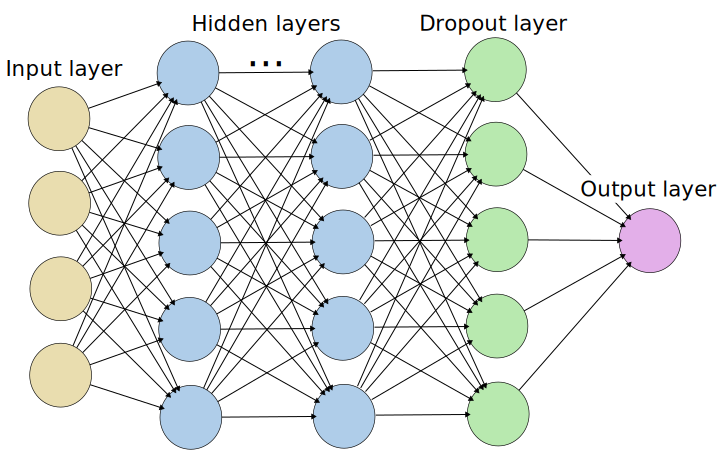
\includegraphics[width=1\textwidth,height=\textheight]{figures/diagram.png}

}

\caption{\label{fig-diagram}A diagram of a feedforward neural network
using densely connected layers.}

\end{figure}

We can also visualize this specific model, using the
\texttt{plot\_model()} function from \texttt{keras.utils}. This function
will give us the schematic in Figure~\ref{fig-model}, showing the type
of layers we're using (either ``InputLayer'', ``Dense'', or
``Dropout''), the activation function in use (either ``relu'' or
``sigmoid''), the number of inputs to each neuron in the layer, and the
number of outputs generated by the layer.

\begin{Shaded}
\begin{Highlighting}[]
\NormalTok{shrubland\_model }\OperatorTok{=}\NormalTok{ make\_model()}

\NormalTok{keras.utils.plot\_model(}
\NormalTok{  shrubland\_model, show\_shapes}\OperatorTok{=}\VariableTok{True}\NormalTok{, show\_layer\_activations}\OperatorTok{=}\VariableTok{True}\NormalTok{, dpi}\OperatorTok{=}\DecValTok{1200}
\NormalTok{)}
\end{Highlighting}
\end{Shaded}

\begin{figure}[H]

{\centering \includegraphics{earth-science-ai-shrubland_files/figure-pdf/fig-model-output-1.png}

}

\caption{\label{fig-model}A schematic showing the structure of our
neural network.}

\end{figure}

As we're fitting a rather deep neural network against rather simple
structured data, we need to be careful to avoid overfitting while we
train the model. As a result, we should define a way to stop our
training process early once we stop seeing improved accuracy against the
validation data set. We can use the \texttt{EarlyStopping()} function to
enforce this behavior, so that we'll cut the training process short once
we stop seeing improvements in PRC against the validation data:

\begin{Shaded}
\begin{Highlighting}[]
\NormalTok{early\_stopping }\OperatorTok{=}\NormalTok{ tf.keras.callbacks.EarlyStopping(}
\NormalTok{    monitor}\OperatorTok{=}\StringTok{"val\_PRC"}\NormalTok{, verbose}\OperatorTok{=}\DecValTok{1}\NormalTok{, patience}\OperatorTok{=}\DecValTok{10}\NormalTok{, mode}\OperatorTok{=}\StringTok{"max"}\NormalTok{, restore\_best\_weights}\OperatorTok{=}\VariableTok{True}
\NormalTok{)}
\end{Highlighting}
\end{Shaded}

And now we're ready to fit the model! Because we're using early
stopping, we can set the number of epochs to use extremely high, as
we'll automatically use the most successful iteration for our final
model. We'll also make sure to use the class weights we defined earlier:

\begin{Shaded}
\begin{Highlighting}[]
\NormalTok{resampled\_history }\OperatorTok{=}\NormalTok{ shrubland\_model.fit(}
\NormalTok{    train\_ds,}
\NormalTok{    steps\_per\_epoch}\OperatorTok{=}\DecValTok{20}\NormalTok{,}
\NormalTok{    epochs}\OperatorTok{=}\DecValTok{1000}\NormalTok{,}
\NormalTok{    callbacks}\OperatorTok{=}\NormalTok{[early\_stopping],}
\NormalTok{    validation\_data}\OperatorTok{=}\NormalTok{(val\_ds),}
\NormalTok{    class\_weight}\OperatorTok{=}\NormalTok{class\_weight,}
\NormalTok{    verbose}\OperatorTok{=}\DecValTok{0}\NormalTok{,}
\NormalTok{)}
\end{Highlighting}
\end{Shaded}

\begin{verbatim}
Restoring model weights from the end of the best epoch: 36.
\end{verbatim}

\begin{verbatim}
Epoch 46: early stopping
\end{verbatim}

It appears that our model's PRC score stops improving after 36 epochs,
which due to our ``patience'' value of 10 causes our early stopping
rules to kick in after epoch 46. We can visualize this process by
plotting the PRC values from each epoch of model training, using the
\texttt{resampled\_history} object returned from the fitting process:

\begin{Shaded}
\begin{Highlighting}[]
\ImportTok{import}\NormalTok{ matplotlib.pyplot }\ImportTok{as}\NormalTok{ plt}

\NormalTok{plt.plot(resampled\_history.history[}\StringTok{"PRC"}\NormalTok{], label}\OperatorTok{=}\StringTok{"PRC (training data)"}\NormalTok{)}
\NormalTok{plt.plot(resampled\_history.history[}\StringTok{"val\_PRC"}\NormalTok{], label}\OperatorTok{=}\StringTok{"PRC (validation data)"}\NormalTok{)}
\NormalTok{plt.ylabel(}\StringTok{"Metric value"}\NormalTok{)}
\NormalTok{plt.xlabel(}\StringTok{"Epoch number"}\NormalTok{)}
\NormalTok{plt.legend(loc}\OperatorTok{=}\StringTok{"upper left"}\NormalTok{)}
\NormalTok{plt.show()}
\end{Highlighting}
\end{Shaded}

\begin{figure}[H]

{\centering \includegraphics{earth-science-ai-shrubland_files/figure-pdf/fig-training-output-1.pdf}

}

\caption{\label{fig-training}Precision-recall curve (PRC) at each epoch
of model training. Higher PRC values indicate a better classifier.}

\end{figure}

This graph (Figure~\ref{fig-training}) provides more information about
the model fitting process than simply knowing when our early stopping
rules kicked in.

It appears that, even though our highest PRC score was achieved after 36
epochs, we might have achieved even higher PRC values had early stopping
not kicked in.

For the purposes of this tutorial, we're going to continue using the
model produced after 36 epochs. Later, as part of the Assignment section
of the chapter, you might want to try other parameters in the early
stopping function to see if you can improve the performance of the
model.

\hypertarget{model-evaluation}{%
\subsection{Model Evaluation}\label{model-evaluation}}

And just like that, we have a neural net trained to identify shrubland!
Now that our model is fully trained (after 36 epochs), the next step is
to evaluate it against our hold-out test data frame. We can use the
\texttt{evaluate()} method of our model object to do so:

\begin{Shaded}
\begin{Highlighting}[]
\NormalTok{results }\OperatorTok{=}\NormalTok{ shrubland\_model.evaluate(test\_ds, verbose}\OperatorTok{=}\DecValTok{0}\NormalTok{)}

\ControlFlowTok{for}\NormalTok{ name, value }\KeywordTok{in} \BuiltInTok{zip}\NormalTok{(shrubland\_model.metrics\_names, results):}
    \BuiltInTok{print}\NormalTok{(name, }\StringTok{": "}\NormalTok{, value)}
\BuiltInTok{print}\NormalTok{()}
\end{Highlighting}
\end{Shaded}

\begin{verbatim}
loss :  0.360729843378067
True_Positives :  17973.0
False_Positives :  289779.0
True_Negatives :  1121321.0
False_Negatives :  3968.0
Binary_Accuracy :  0.7950184345245361
Precision :  0.058400921523571014
Recall :  0.8191513419151306
AUC :  0.8857248425483704
PRC :  0.1751827746629715
\end{verbatim}

We'll discuss these results in more detail in the Discussion
(Section~\ref{sec-discussion}). For now, though, make note of how high
our model's AUC (area under the ROC curve) is, compared to its PRC (area
under the precision-recall curve) and precision.

Last but not least, it's time for us to visualize our predictions to get
a sense of where our model believes we're most likely to find
shrublands. In order to map our results, we need to first generate a
prediction for each cell in our raster. To do that, we need to first
pre-process our full data set in the same way as our training and test
data by rescaling it and transforming it to a TensorFlow dataset:

\begin{Shaded}
\begin{Highlighting}[]
\NormalTok{full\_array }\OperatorTok{=}\NormalTok{ np.array(full\_features)}
\NormalTok{full\_array }\OperatorTok{=}\NormalTok{ scaler.transform(full\_array)}

\NormalTok{full\_ds }\OperatorTok{=}\NormalTok{ tf.data.Dataset.from\_tensor\_slices((full\_array, full\_labels)).cache()}
\NormalTok{full\_ds }\OperatorTok{=}\NormalTok{ full\_ds.batch(}\DecValTok{64}\NormalTok{).prefetch(}\DecValTok{2}\NormalTok{)}
\end{Highlighting}
\end{Shaded}

We can then generate a prediction for each cell of our raster using our
model's \texttt{predict()} method:

\begin{Shaded}
\begin{Highlighting}[]
\NormalTok{predictions }\OperatorTok{=}\NormalTok{ pd.DataFrame(shrubland\_model.predict(full\_ds, verbose}\OperatorTok{=}\DecValTok{0}\NormalTok{))}

\NormalTok{full\_data }\OperatorTok{=}\NormalTok{ pd.concat(}
\NormalTok{    [full\_data, predictions],}
\NormalTok{    axis}\OperatorTok{=}\DecValTok{1}\NormalTok{,}
\NormalTok{)}
\end{Highlighting}
\end{Shaded}

Now all that's left is to save our predictions out as a raster file, so
that we can visualize them in our favorite GIS tool. In order to save
space, we'll only save our X and Y coordinates and predictions in the
output raster, producing a simple XYZ raster file:

\begin{Shaded}
\begin{Highlighting}[]
\NormalTok{location\_predictions }\OperatorTok{=}\NormalTok{ full\_data[[}\StringTok{"x"}\NormalTok{, }\StringTok{"y"}\NormalTok{, }\DecValTok{0}\NormalTok{]]}
\NormalTok{location\_predictions.columns }\OperatorTok{=}\NormalTok{ [}\StringTok{"x"}\NormalTok{, }\StringTok{"y"}\NormalTok{, }\StringTok{"z"}\NormalTok{]}
\end{Highlighting}
\end{Shaded}

We'll use \texttt{rasterio} in order to save this out as a raster file
that GIS tools will understand. Let's import it (and its dependency,
\texttt{affine}) now:

\begin{Shaded}
\begin{Highlighting}[]
\ImportTok{import}\NormalTok{ rasterio}
\ImportTok{from}\NormalTok{ affine }\ImportTok{import}\NormalTok{ Affine}
\end{Highlighting}
\end{Shaded}

A raster file is effectively an array of values, with each cell's X and
Y position in the array corresponding to its X and Y position in space.
As such, in order to create a raster file we must first transpose our
one-dimensional column of predictions into a two-dimensional array.

Our first step in this process is to find the corners of our data's
bounding box:

\begin{Shaded}
\begin{Highlighting}[]
\NormalTok{xmin }\OperatorTok{=}\NormalTok{ location\_predictions[}\StringTok{"x"}\NormalTok{].}\BuiltInTok{min}\NormalTok{()}
\NormalTok{xmax }\OperatorTok{=}\NormalTok{ location\_predictions[}\StringTok{"x"}\NormalTok{].}\BuiltInTok{max}\NormalTok{()}
\NormalTok{ymin }\OperatorTok{=}\NormalTok{ location\_predictions[}\StringTok{"y"}\NormalTok{].}\BuiltInTok{min}\NormalTok{()}
\NormalTok{ymax }\OperatorTok{=}\NormalTok{ location\_predictions[}\StringTok{"y"}\NormalTok{].}\BuiltInTok{max}\NormalTok{()}
\end{Highlighting}
\end{Shaded}

We then need to identify the cell positions of each pixel in our data
set:

\begin{Shaded}
\begin{Highlighting}[]
\CommentTok{\# Resolution of our Landsat{-}derived predictors:}
\CommentTok{\# Each observation represents a 30{-}meter square "pixel" of the map}
\NormalTok{pixel\_size }\OperatorTok{=} \DecValTok{30}

\CommentTok{\# Identify the X and Y values for each pixel in our output raster}
\NormalTok{xv }\OperatorTok{=}\NormalTok{ pd.Series(np.arange(xmin, xmax }\OperatorTok{+}\NormalTok{ pixel\_size, pixel\_size))}
\NormalTok{yv }\OperatorTok{=}\NormalTok{ pd.Series(np.arange(ymin, ymax }\OperatorTok{+}\NormalTok{ pixel\_size, pixel\_size)[::}\OperatorTok{{-}}\DecValTok{1}\NormalTok{])}

\CommentTok{\# Get the X and Y cell indices for each of these pixels}
\NormalTok{xi }\OperatorTok{=}\NormalTok{ pd.Series(xv.index.values, index}\OperatorTok{=}\NormalTok{xv)}
\NormalTok{yi }\OperatorTok{=}\NormalTok{ pd.Series(yv.index.values, index}\OperatorTok{=}\NormalTok{yv)}
\end{Highlighting}
\end{Shaded}

And we'll then use those positions to create an empty array, which we'll
then fill in with our predicted values:

\begin{Shaded}
\begin{Highlighting}[]
\CommentTok{\# Create an empty array of the proper size for our data:}
\NormalTok{nodata }\OperatorTok{=} \OperatorTok{{-}}\FloatTok{9999.0}
\NormalTok{zv }\OperatorTok{=}\NormalTok{ np.ones((}\BuiltInTok{len}\NormalTok{(yi), }\BuiltInTok{len}\NormalTok{(xi)), np.float32) }\OperatorTok{*}\NormalTok{ nodata}

\CommentTok{\# Fill in the array with our predicted values, wherever they exist:}
\NormalTok{zv[}
\NormalTok{    yi[location\_predictions[}\StringTok{"y"}\NormalTok{]].values, xi[location\_predictions[}\StringTok{"x"}\NormalTok{]].values}
\NormalTok{] }\OperatorTok{=}\NormalTok{ location\_predictions[}\StringTok{"z"}\NormalTok{]}
\end{Highlighting}
\end{Shaded}

And just like that, we've transformed our single-dimension prediction
vector into a two-dimensional array. All that remains is to translate
that array from a numpy array into a raster file. We'll first define a
transformation, to give rasterio instructions on how much area each of
our array cells should represent:

\begin{Shaded}
\begin{Highlighting}[]
\NormalTok{transform }\OperatorTok{=}\NormalTok{ Affine(pixel\_size, }\DecValTok{0}\NormalTok{, xmin, }\DecValTok{0}\NormalTok{, }\OperatorTok{{-}}\NormalTok{pixel\_size, ymax) }\OperatorTok{*}\NormalTok{ Affine.translation(}
    \OperatorTok{{-}}\FloatTok{0.5}\NormalTok{, }\OperatorTok{{-}}\FloatTok{0.5}
\NormalTok{)}
\end{Highlighting}
\end{Shaded}

And then lastly we'll use rasterio and this transformation to actually
write our values out to a GeoTIFF file:

\begin{Shaded}
\begin{Highlighting}[]
\CommentTok{\# This is the PROJ string for the raster data used in this study}
\CommentTok{\# It represents how to associate the X and Y coordinates with real world data}
\NormalTok{projection }\OperatorTok{=} \StringTok{"+proj=aea +lat\_0=23 +lon\_0={-}96 +lat\_1=29.5 +lat\_2=45.5"}
\NormalTok{projection }\OperatorTok{=}\NormalTok{ projection }\OperatorTok{+} \StringTok{" +x\_0=0 +y\_0=0 +datum=WGS84 +units=m +no\_defs"}

\ControlFlowTok{with}\NormalTok{ rasterio.}\BuiltInTok{open}\NormalTok{(}
    \CommentTok{\# Our output file name}
    \StringTok{"predictions.tiff"}\NormalTok{,}
    \CommentTok{\# What mode to open the file in {-}{-} here, write mode}
    \StringTok{"w"}\NormalTok{,}
    \CommentTok{\# What driver to use to write our file}
    \StringTok{"GTiff"}\NormalTok{,}
    \CommentTok{\# Number of columns to write}
    \BuiltInTok{len}\NormalTok{(xi),}
    \CommentTok{\# Number of rows to write}
    \BuiltInTok{len}\NormalTok{(yi),}
    \CommentTok{\# How many "bands" to write}
    \DecValTok{1}\NormalTok{,}
\NormalTok{    projection,}
    \CommentTok{\# The transformation created above}
\NormalTok{    transform,}
    \CommentTok{\# What data type to save as}
\NormalTok{    rasterio.float32,}
    \CommentTok{\# What value indicates a missing value}
\NormalTok{    nodata,}
\NormalTok{) }\ImportTok{as}\NormalTok{ ds:}
\NormalTok{    ds.write(zv.astype(np.float32), }\DecValTok{1}\NormalTok{)}
\end{Highlighting}
\end{Shaded}

Once we've saved this GeoTIFF file, we can visualize it in any GIS
program to see where our model predicts shrubland is located
(Figure~\ref{fig-predictions}).

\begin{figure}

{\centering 

\includegraphics{figures/model_predictions.png}

}

\caption{\label{fig-predictions}A map of predicted probability of
shrubland occurance across New York's lower Hudson River valley,
including Duchess, Orange and Ulster counties.}

\end{figure}

\hypertarget{sec-discussion}{%
\section{Discussion}\label{sec-discussion}}

So we've fit our models, predicted our data, and made a map of the
results. But what do our results actually mean, both for our ability to
identify shrubland and for how we understand model performance?

A lot of researchers are immediately drawn to the best performance
metrics of the model -- in this case, likely our fantastic AUC
statistic. However, remember that our data is severely imbalanced, with
only 1.5\% of the training data representing shrublands. AUC is a
measure of how well your model performs at the ``pairing test'' -- that
is, it represents how well our model would do at classifying two
observations if one was guaranteed to represent shrubland and one was
guaranteed to not (Hand 2009).

In that situation, our model would give the right results 89\% of the
time, which makes it a highly effective classifier. However, given that
only 1.5\% of our region is shrubland, the scenario described by AUC
isn't a great representation of how our model actually performs on the
ground.

More interesting are our model's recall and precision scores. Our recall
score -- that is, the proportion of actual ``true'' shrublands which the
model calls shrubland -- is extremely high for this model. Our model
produces very few false negative predictions. However, our precision --
the proportion of shrubland predictions which actually reflect ``true''
shrubland -- is much lower, as we have a very high number of false
positives. Depending on our goals for this model, this may be desirable;
if our aim is to identify the majority of shrubland across the state, we
may accept these false positives as a necessary drawback of that goal.
However, if our goal is to produce the most accurate map of shrubland
locations possible, for instance to try and choose sites for fieldwork
in shrubland regions, we might want a higher precision in exchange for a
lower recall value.

Because our model predicts the probability that an observation
represents shrubland, and not just the class, we can use different
classification thresholds to balance recall and precision according to
our tastes. For instance, we can see a large increase in model precision
if we require a predicted probability of more than 90\% before we
classify an observation as shrubland:

\begin{Shaded}
\begin{Highlighting}[]
\NormalTok{test\_predictions }\OperatorTok{=}\NormalTok{ pd.DataFrame(shrubland\_model.predict(test\_ds, verbose}\OperatorTok{=}\DecValTok{0}\NormalTok{))}

\ImportTok{import}\NormalTok{ statistics}

\NormalTok{statistics.mean(test\_labels.loc[np.array(test\_predictions[}\DecValTok{0}\NormalTok{] }\OperatorTok{\textgreater{}} \FloatTok{0.9}\NormalTok{)])}
\end{Highlighting}
\end{Shaded}

\begin{verbatim}
0.5772755039706781
\end{verbatim}

And an even bigger improvement if we require a probability of at least
95\%:

\begin{Shaded}
\begin{Highlighting}[]
\NormalTok{statistics.mean(test\_labels.loc[np.array(test\_predictions[}\DecValTok{0}\NormalTok{] }\OperatorTok{\textgreater{}} \FloatTok{0.95}\NormalTok{)])}
\end{Highlighting}
\end{Shaded}

\begin{verbatim}
0.8323932312651088
\end{verbatim}

Of course, this improved precision comes at the cost of a decrease in
recall. This is a common trade-off with classification models:
decreasing the number of false positives also decreases the number of
true positives predicted by a given model. The appropriate threshold to
use when making predictions for any classifier will be dependent upon
the relative costs of false negative and false positive predictions for
your use case.

Perhaps more interesting than the specific probability predictions is
the spatial arrangement of predictions across our study area
(Figure~\ref{fig-predictions}). Generally speaking, it appears like our
model is expecting shrubland to be more dominant in areas along road
networks and rivers (which are white in the map, as they were excluded
from our input data set) -- which makes a lot of sense, as these are the
areas more likely to have been recently impacted by humans. In this way,
mapping the results of a predictive model can help us to understand the
patterns and processes happening across the landscape, even without the
use of an inferential or causal framework. Being able to visualize what
areas are more likely to be shrubland, in this scenario, can help us
generate hypotheses for why shrubland occurs where it does and perhaps
even suggest future areas for inferential investigation.

\hypertarget{summary}{%
\section{Summary}\label{summary}}

This chapter provided a step-by-step walk through of the process for
producing models of a rare land-cover class, using a case study
attempting to identify shrublands across a region in New York State. Due
to the rarity of shrublands in this region, specific attention was paid
to how to model imbalanced classes and how to measure model performance
with specific objectives for the model. While our model was better at
identifying shrubland than random chance alone (with a precision
multiple times greater than the 1.5\% ``base rate'' of all pixels being
shrubland), the rarity of this land cover class means that the model's
precision is rather low in absolute terms. As higher predicted
probabilities of shrubland are, as expected, more likely to represent
actual shrubland areas, adjusting the classification threshold to
require higher probabilities can help to improve model performance.

More generally, this chapter focused on the difficulties of modeling
rare events, and approaches that can be used in this common situation.
It is frequently true that rare events and abnormalities are more
scientifically interesting than the baseline case, and as such it is
important to be able to model and predict these situations. By being
able to assign class weights and thinking carefully about model
performance metrics, we're able to apply most modeling tools to this
common type of problem.

\hypertarget{assignment}{%
\section{Assignment}\label{assignment}}

\begin{itemize}
\tightlist
\item
  Try altering the architecture of the neural network -- remove layers,
  change the number of nodes, alter the early stopping callback, and
  generally play with the form of the model. Can you out-perform the
  model from the chapter?
\item
  What happens if you use a different metric for early stopping? Can you
  optimize for a different performance metric?
\item
  What happens if you change the class weights to more strongly
  emphasize shrublands? To de-emphasize them? What metrics are impacted
  the most?
\end{itemize}

\hypertarget{open-questions}{%
\section{Open Questions}\label{open-questions}}

There remain some clear future directions for this model:

\begin{itemize}
\tightlist
\item
  Could additional predictors (derived from Landsat imagery or other
  remote sensing data sources) improve predictive accuracy?
\item
  Could this model be used to track the development of shrubland areas
  over time, in order to monitor the abundance and distribution of this
  land cover type?
\item
  Will the reported performance statistics remain stable as the model is
  used to extrapolate into other regions of New York? Into other regions
  of the country?
\item
  Could a similar approach be used to track other novel land cover
  classes, or a finer gradation of land cover types than is usually
  modeled in LULC studies?
\item
  Could more complex models, such as convolutional neural networks,
  achieve higher accuracy against this data set?
\end{itemize}

\newpage{}

\hypertarget{references}{%
\section*{References}\label{references}}
\addcontentsline{toc}{section}{References}

\hypertarget{refs}{}
\begin{CSLReferences}{1}{0}
\leavevmode\vadjust pre{\hypertarget{ref-tensorflow}{}}%
Abadi, Martín, Ashish Agarwal, Paul Barham, Eugene Brevdo, Zhifeng Chen,
Craig Citro, Greg S. Corrado, et al. 2015. {``{TensorFlow}: Large-Scale
Machine Learning on Heterogeneous Systems.''}
\url{https://www.tensorflow.org/}.

\leavevmode\vadjust pre{\hypertarget{ref-LCMAP}{}}%
Brown, Jesslyn F., Heather J. Tollerud, Christopher P. Barber, Qiang
Zhou, John L. Dwyer, James E. Vogelmann, Thomas R. Loveland, et al.
2020. {``Lessons Learned Implementing an Operational Continuous United
States National Land Change Monitoring Capability: The Land Change
Monitoring, Assessment, and Projection (LCMAP) Approach.''} \emph{Remote
Sensing of Environment} 238: 111356.
\url{https://doi.org/10.1016/j.rse.2019.111356}.

\leavevmode\vadjust pre{\hypertarget{ref-pydot}{}}%
Carrera, Ero, Peter Nowee, and Sebastian Kalinowski. 2021. \emph{Pydot}.
\url{https://github.com/pydot/pydot}.

\leavevmode\vadjust pre{\hypertarget{ref-keras}{}}%
Chollet, François. 2015. {``Keras.''} \url{https://keras.io}.

\leavevmode\vadjust pre{\hypertarget{ref-Cramer2008}{}}%
Cramer, Viki A, Richard J Hobbs, and Rachel J Standish. 2008. {``What's
New about Old Fields? Land Abandonment and Ecosystem Assembly.''}
\emph{Trends in Ecology \& Evolution} 23 (2): 104--12.
\url{https://doi.org/10.1016/j.tree.2007.10.005}.

\leavevmode\vadjust pre{\hypertarget{ref-Falkowski2009}{}}%
Falkowski, Michael J., Jeffrey S. Evans, Sebastian Martinuzzi, Paul E.
Gessler, and Andrew T. Hudak. 2009. {``Characterizing Forest Succession
with Lidar Data: An Evaluation for the Inland Northwest, USA.''}
\emph{Remote Sensing of Environment} 113 (5): 946--56.
https://doi.org/\url{https://doi.org/10.1016/j.rse.2009.01.003}.

\leavevmode\vadjust pre{\hypertarget{ref-Fargione2018}{}}%
Fargione, Joseph E, Steven Bassett, Timothy Boucher, Scott D Bridgham,
Richard T Conant, Susan C Cook-Patton, Peter W Ellis, et al. 2018.
{``Natural Climate Solutions for the United States.''} \emph{Science
Advances} 4 (11): eaat1869.
\url{https://doi.org/10.1126/sciadv.aat1869}.

\leavevmode\vadjust pre{\hypertarget{ref-Foster1998}{}}%
Foster, David R, Glenn Motzkin, and Benjamin Slater. 1998. {``Land-Use
History as Long-Term Broad-Scale Disturbance: Regional Forest Dynamics
in Central New England.''} \emph{Ecosystems} 1 (1): 96--119.
\url{https://doi.org/10.1007/s100219900008}.

\leavevmode\vadjust pre{\hypertarget{ref-gillies_2019}{}}%
Gillies, Sean et al. 2013. \emph{Rasterio: Geospatial Raster i/o for
{Python} Programmers}. Mapbox.
\url{https://github.com/rasterio/rasterio}.

\leavevmode\vadjust pre{\hypertarget{ref-Hand2009}{}}%
Hand, David J. 2009. {``Measuring Classifier Performance: A Coherent
Alternative to the Area Under the ROC Curve.''} \emph{Machine Learning}
77: 103--23.

\leavevmode\vadjust pre{\hypertarget{ref-harris2020array}{}}%
Harris, Charles R., K. Jarrod Millman, Stéfan J. van der Walt, Ralf
Gommers, Pauli Virtanen, David Cournapeau, Eric Wieser, et al. 2020.
{``Array Programming with {NumPy}.''} \emph{Nature} 585 (7825): 357--62.
\url{https://doi.org/10.1038/s41586-020-2649-2}.

\leavevmode\vadjust pre{\hypertarget{ref-Hobbs2009}{}}%
Hobbs, Richard J, Eric Higgs, and James A Harris. 2009. {``Novel
Ecosystems: Implications for Conservation and Restoration.''}
\emph{Trends in Ecology \& Evolution} 24 (11): 599--605.
\url{https://doi.org/10.1016/j.tree.2009.05.012}.

\leavevmode\vadjust pre{\hypertarget{ref-matplotlib}{}}%
Hunter, J. D. 2007. {``Matplotlib: A 2d Graphics Environment.''}
\emph{Computing in Science \& Engineering} 9 (3): 90--95.
\url{https://doi.org/10.1109/MCSE.2007.55}.

\leavevmode\vadjust pre{\hypertarget{ref-Kennedy2010}{}}%
Kennedy, Robert E, Zhiqiang Yang, and Warren B. Cohen. 2010.
{``Detecting Trends in Forest Disturbance and Recovery Using Yearly
Landsat Time Series: 1. {LandTrendr} {\textemdash} Temporal Segmentation
Algorithms.''} \emph{Remote Sensing of Environment} 114 (12):
2897--2910. \url{https://doi.org/10.1016/j.rse.2010.07.008}.

\leavevmode\vadjust pre{\hypertarget{ref-Kennedy2018}{}}%
Kennedy, Robert E, Zhiqiang Yang, Noel Gorelick, Justin Braaten, Lucas
Cavalcante, Warren B. Cohen, and Sean Healey. 2018. {``Implementation of
the LandTrendr Algorithm on Google Earth Engine.''} \emph{Remote
Sensing} 10 (5). \url{https://doi.org/10.3390/rs10050691}.

\leavevmode\vadjust pre{\hypertarget{ref-King2014}{}}%
King, David I., and Scott Schlossberg. 2014. {``Synthesis of the
Conservation Value of the Early-Successional Stage in Forests of Eastern
North America.''} \emph{Forest Ecology and Management} 324: 186--95.
\url{https://doi.org/10.1016/j.foreco.2013.12.001}.

\leavevmode\vadjust pre{\hypertarget{ref-LeCun2015}{}}%
LeCun, Yann, Yoshua Bengio, and Geoffrey Hinton. 2015. {``Deep
Learning.''} \emph{Nature} 521: 436--44.
\url{https://doi.org/10.1038/nature14539}.

\leavevmode\vadjust pre{\hypertarget{ref-Paper}{}}%
Mahoney, Michael J, Lucas K Johnson, and Colin M Beier. 2022a.
{``Classification and Mapping of Low-Statured 'Shrubland' Cover Types in
Post-Agricultural Landscapes of the US Northeast.''} arXiv.
\url{https://doi.org/10.48550/ARXIV.2205.05047}.

\leavevmode\vadjust pre{\hypertarget{ref-data}{}}%
---------. 2022b. {``{Data for: AI for Shrubland Identification and
Mapping (in AI For Earth Science)}.''} Zenodo.
\url{https://doi.org/10.5281/zenodo.6824173}.

\leavevmode\vadjust pre{\hypertarget{ref-mckinney-proc-scipy-2010}{}}%
McKinney, Wes. 2010. {``{D}ata {S}tructures for {S}tatistical
{C}omputing in {P}ython.''} In \emph{{P}roceedings of the 9th {P}ython
in {S}cience {C}onference}, edited by Stéfan van der Walt and Jarrod
Millman, 56--61.
\href{https://doi.org/\%2010.25080/Majora-92bf1922-00a\%20}{https://doi.org/
10.25080/Majora-92bf1922-00a }.

\leavevmode\vadjust pre{\hypertarget{ref-scikit-learn}{}}%
Pedregosa, F., G. Varoquaux, A. Gramfort, V. Michel, B. Thirion, O.
Grisel, M. Blondel, et al. 2011. {``Scikit-Learn: Machine Learning in
{P}ython.''} \emph{Journal of Machine Learning Research} 12: 2825--30.

\leavevmode\vadjust pre{\hypertarget{ref-Python}{}}%
Python Core Team. 2022. \emph{{Python: A dynamic, open source
programming language}}. {Python Software Foundation}.
\url{https://www.python.org/}.

\leavevmode\vadjust pre{\hypertarget{ref-Ruiz2018}{}}%
Ruiz, Luis Ángel, Jorge Abel Recio, Pablo Crespo-Peremarch, and Marta
Sapena. 2018. {``An Object-Based Approach for Mapping Forest Structural
Types Based on Low-Density LiDAR and Multispectral Imagery.''}
\emph{Geocarto International} 33 (5): 443--57.
\url{https://doi.org/10.1080/10106049.2016.1265595}.

\leavevmode\vadjust pre{\hypertarget{ref-reback2020pandas}{}}%
team, The pandas development. 2020. \emph{Pandas-Dev/Pandas: Pandas}
(version latest). Zenodo. \url{https://doi.org/10.5281/zenodo.3509134}.

\leavevmode\vadjust pre{\hypertarget{ref-Wickham2021}{}}%
Wickham, James, Stephen V. Stehman, Daniel G. Sorenson, Leila Gass, and
Jon A. Dewitz. 2021. {``Thematic Accuracy Assessment of the NLCD 2016
Land Cover for the Conterminous United States.''} \emph{Remote Sensing
of Environment} 257: 112357.
https://doi.org/\url{https://doi.org/10.1016/j.rse.2021.112357}.

\end{CSLReferences}



\end{document}
